В этом разделе будут представлены результаты, которые демонстрирует разработанный конвейер, а именно, какое максимальное, минимальное и среднее время тратится на обработку строк длиной $1\:000\:000$ символов, а также анализируется время, которое тратится задачей на ожидание в очереди.

\section{Характеристики ПК}
\qquadПри проведении эксперимента использовался компьютер, имеющий следующие характеристики:
\begin{itemize}
	\item OC - Windows 10 Pro;
	\item процессор - Inter Core i7 10510U (1800 МГц);
	\item объём ОЗУ - 16 Гб;
	\item число логических ядер - 8.
\end{itemize}

\section{Лог конвейерной обработки}
\qquadНа Рисунках \ref{fig8:image}, \ref{fig9:image} приведены результаты обработки 35 задач.

\begin{figure}[h]
	\begin{center}
		{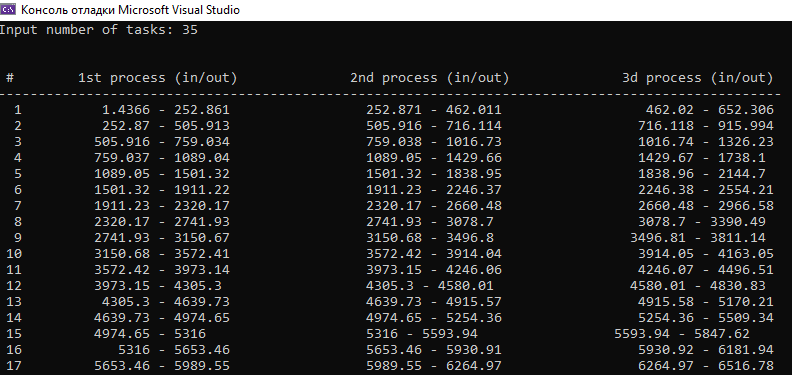
\includegraphics[scale = 0.85]{results/result_1_part_1}}
		\caption{Результаты обработки 35 задач (часть 1)}
		\label{fig8:image}
	\end{center}
\end{figure}

\begin{figure}[h]
	\begin{center}
		{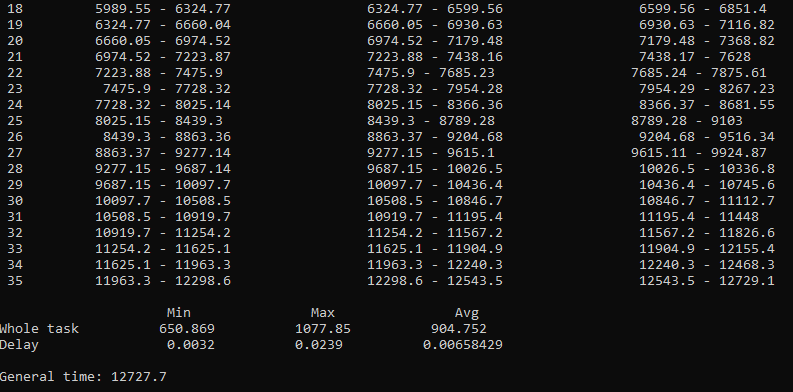
\includegraphics[scale = 0.85]{results/result_1_part_2}}
		\caption{Результаты обработки 35 задач (часть 2)}
		\label{fig9:image}
	\end{center}
\end{figure}

\section*{Выводы}
\addcontentsline{toc}{section}{Вывод}
\qquadСогласно полученным данным, можно сделать следующие \textbf{выводы}.
\begin{itemize}
	\itemСреднее время обработки строк длиной  $1\:000\:000$ символов примерно 904.752 мс, а среднее время ожидания в очереди 0.00658 мс, что составляет меньше 0.0007\% от среднего времени выполнения задачи.
	\itemЕсли рассматривать наибольшие показатели конвейера, то время ожидания будет составлять примерно 0.0022\% от всего времени обработки задачи.
	\itemСоотношение времени ожидания в очереди ко времени выполнения не превышает 0.0037\%.
\end{itemize}
